\documentclass{article}
\usepackage[UTF8]{ctex}
\usepackage{amsmath}
\usepackage{amssymb}
\usepackage{graphicx}
\usepackage{float}
\usepackage{datetime}
\usepackage{geometry}

\geometry{a4paper, top=2.54cm, bottom=2.54cm, left=3.18cm, right=3.18cm}

\author{刘思昀 SLST 2022522011}

\title{General Physics II 磁性材料基本特性的研究}

\begin{document}

\date{\formatdate{10}{4}{2024}}

\maketitle

\section{测绘基本磁化曲线}
\subsection{基本磁化曲线}
将不同$Vpp$下测得的坐标点绘制在同一张图上并连线,得到如下样品的基本磁化曲线:
\begin{figure*}[htbp]
    \centering
    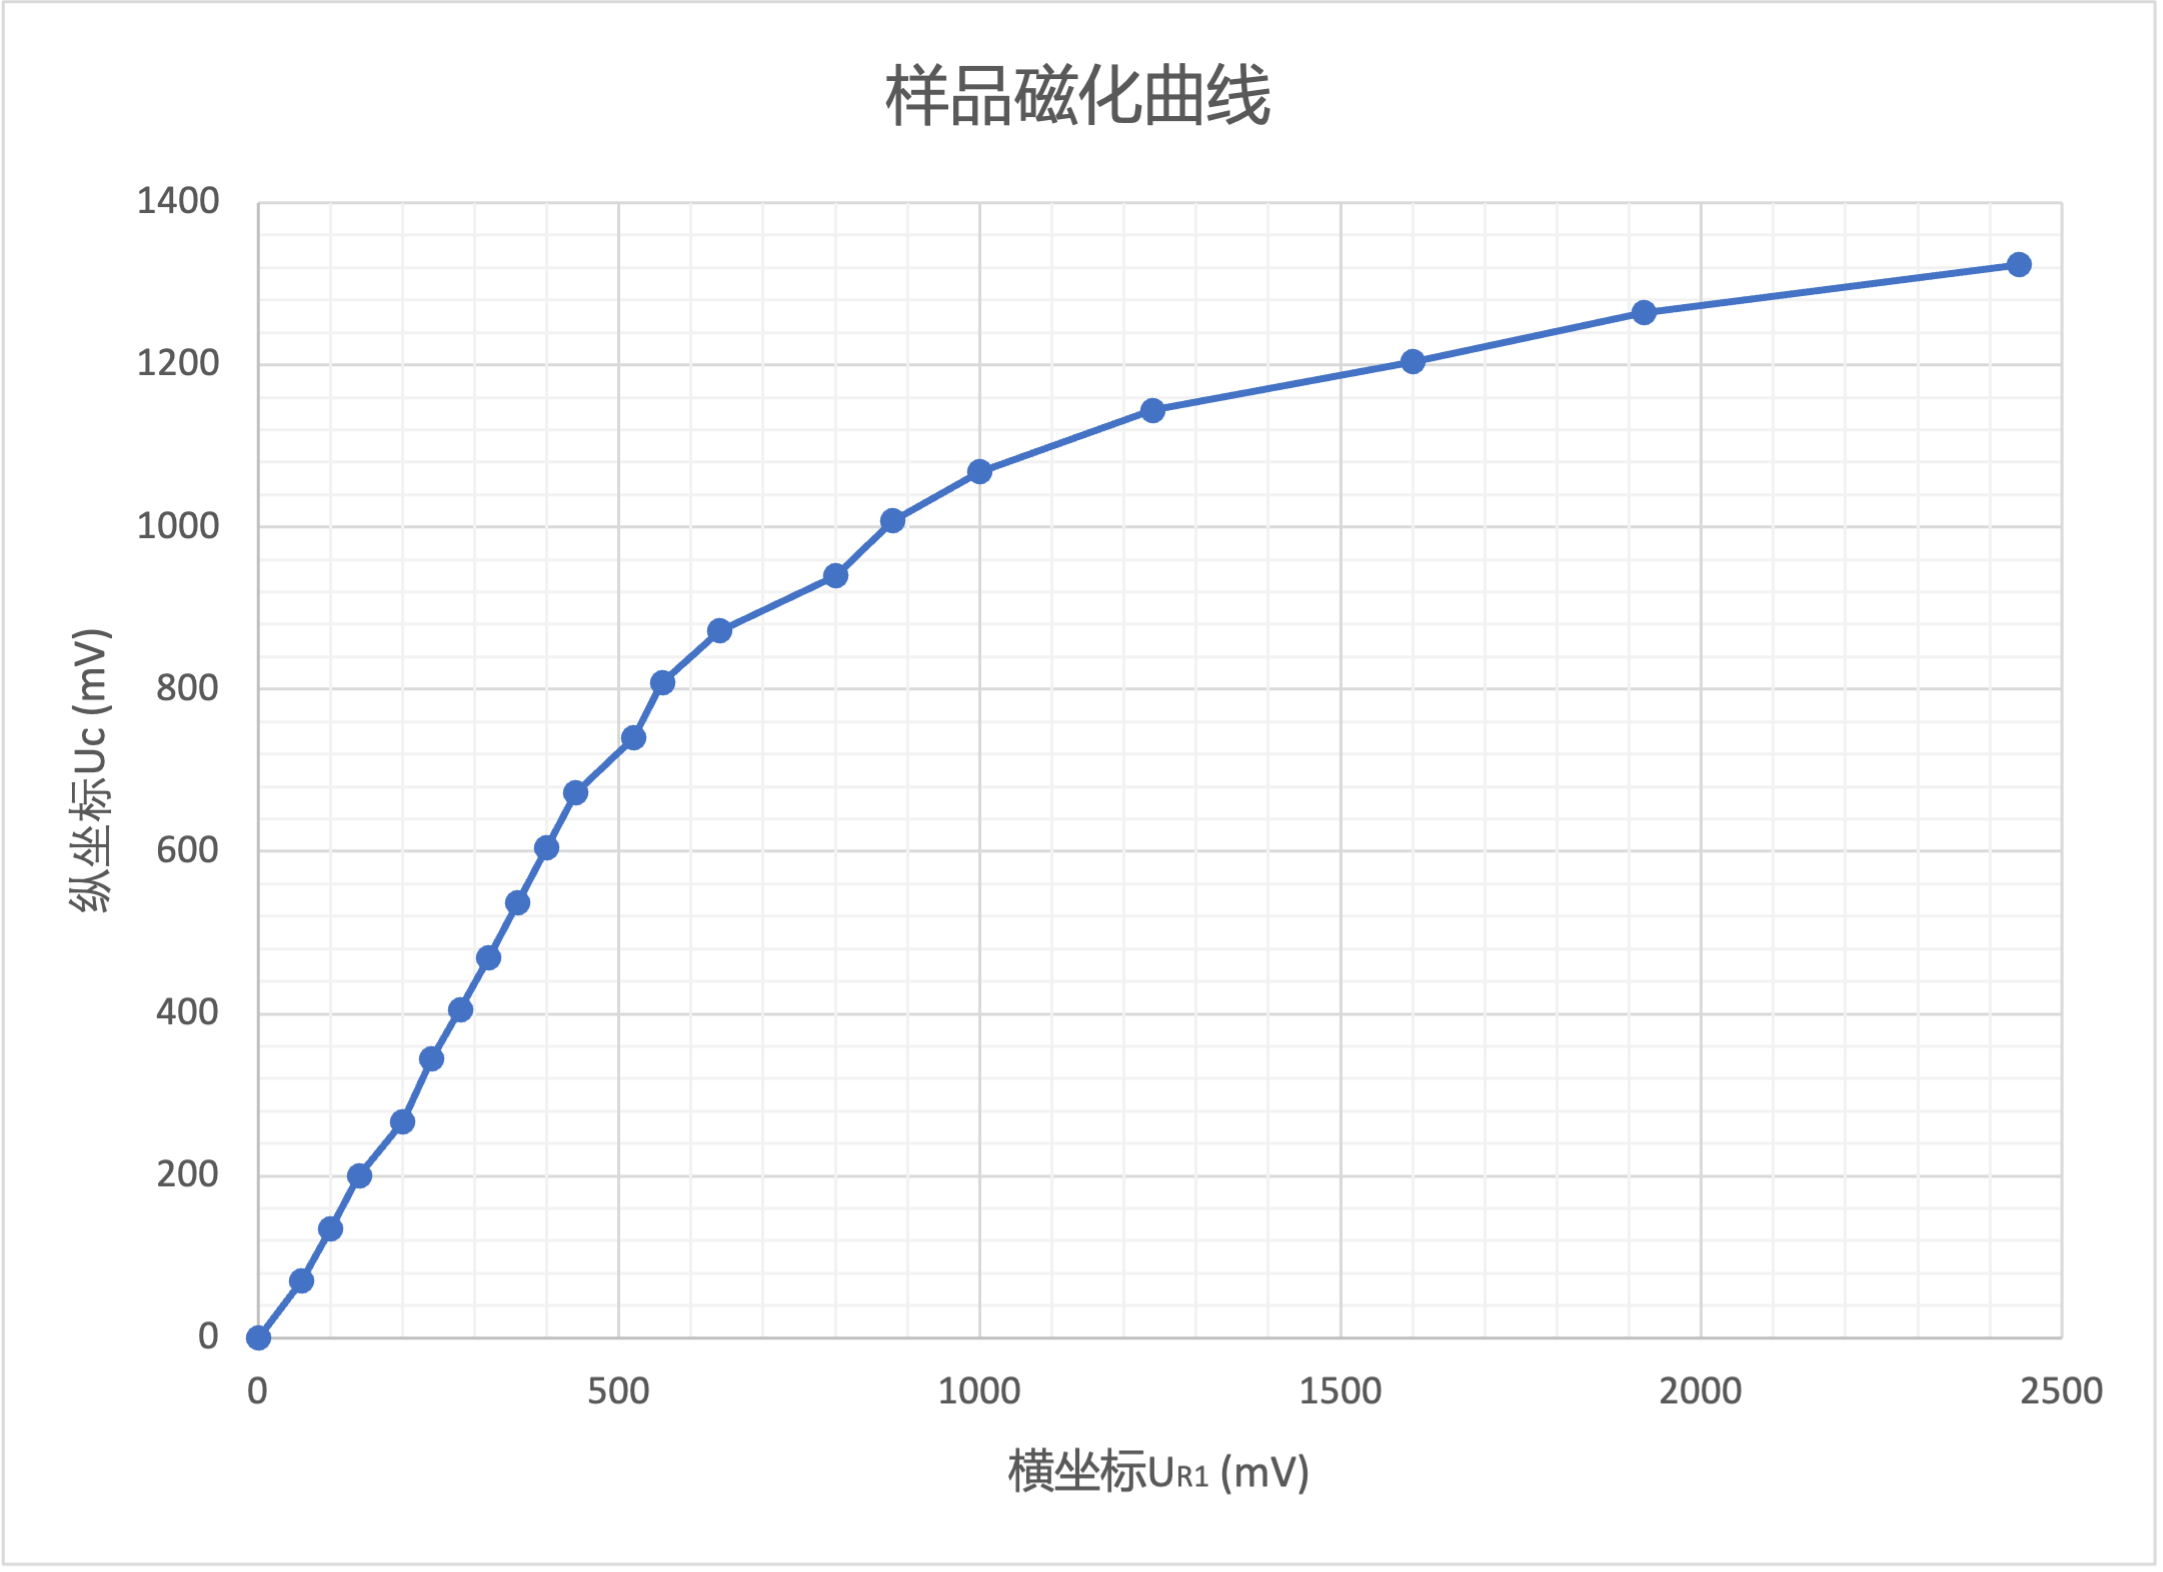
\includegraphics[width=1.0\textwidth]{plot1.png}
    \caption{样品的基本磁化曲线}
\end{figure*}

其中$Vpp = 0V$时,由于无法将信号源直接调至$0V$,故直接将信号源关闭得到结果。

由于讲义中的磁化曲线横纵坐标分别为$H$和$B$,故另外绘制以磁场强度$H$为横坐标,磁感应强度$B$为纵坐标的图像:
\begin{figure*}[htbp]
    \centering
    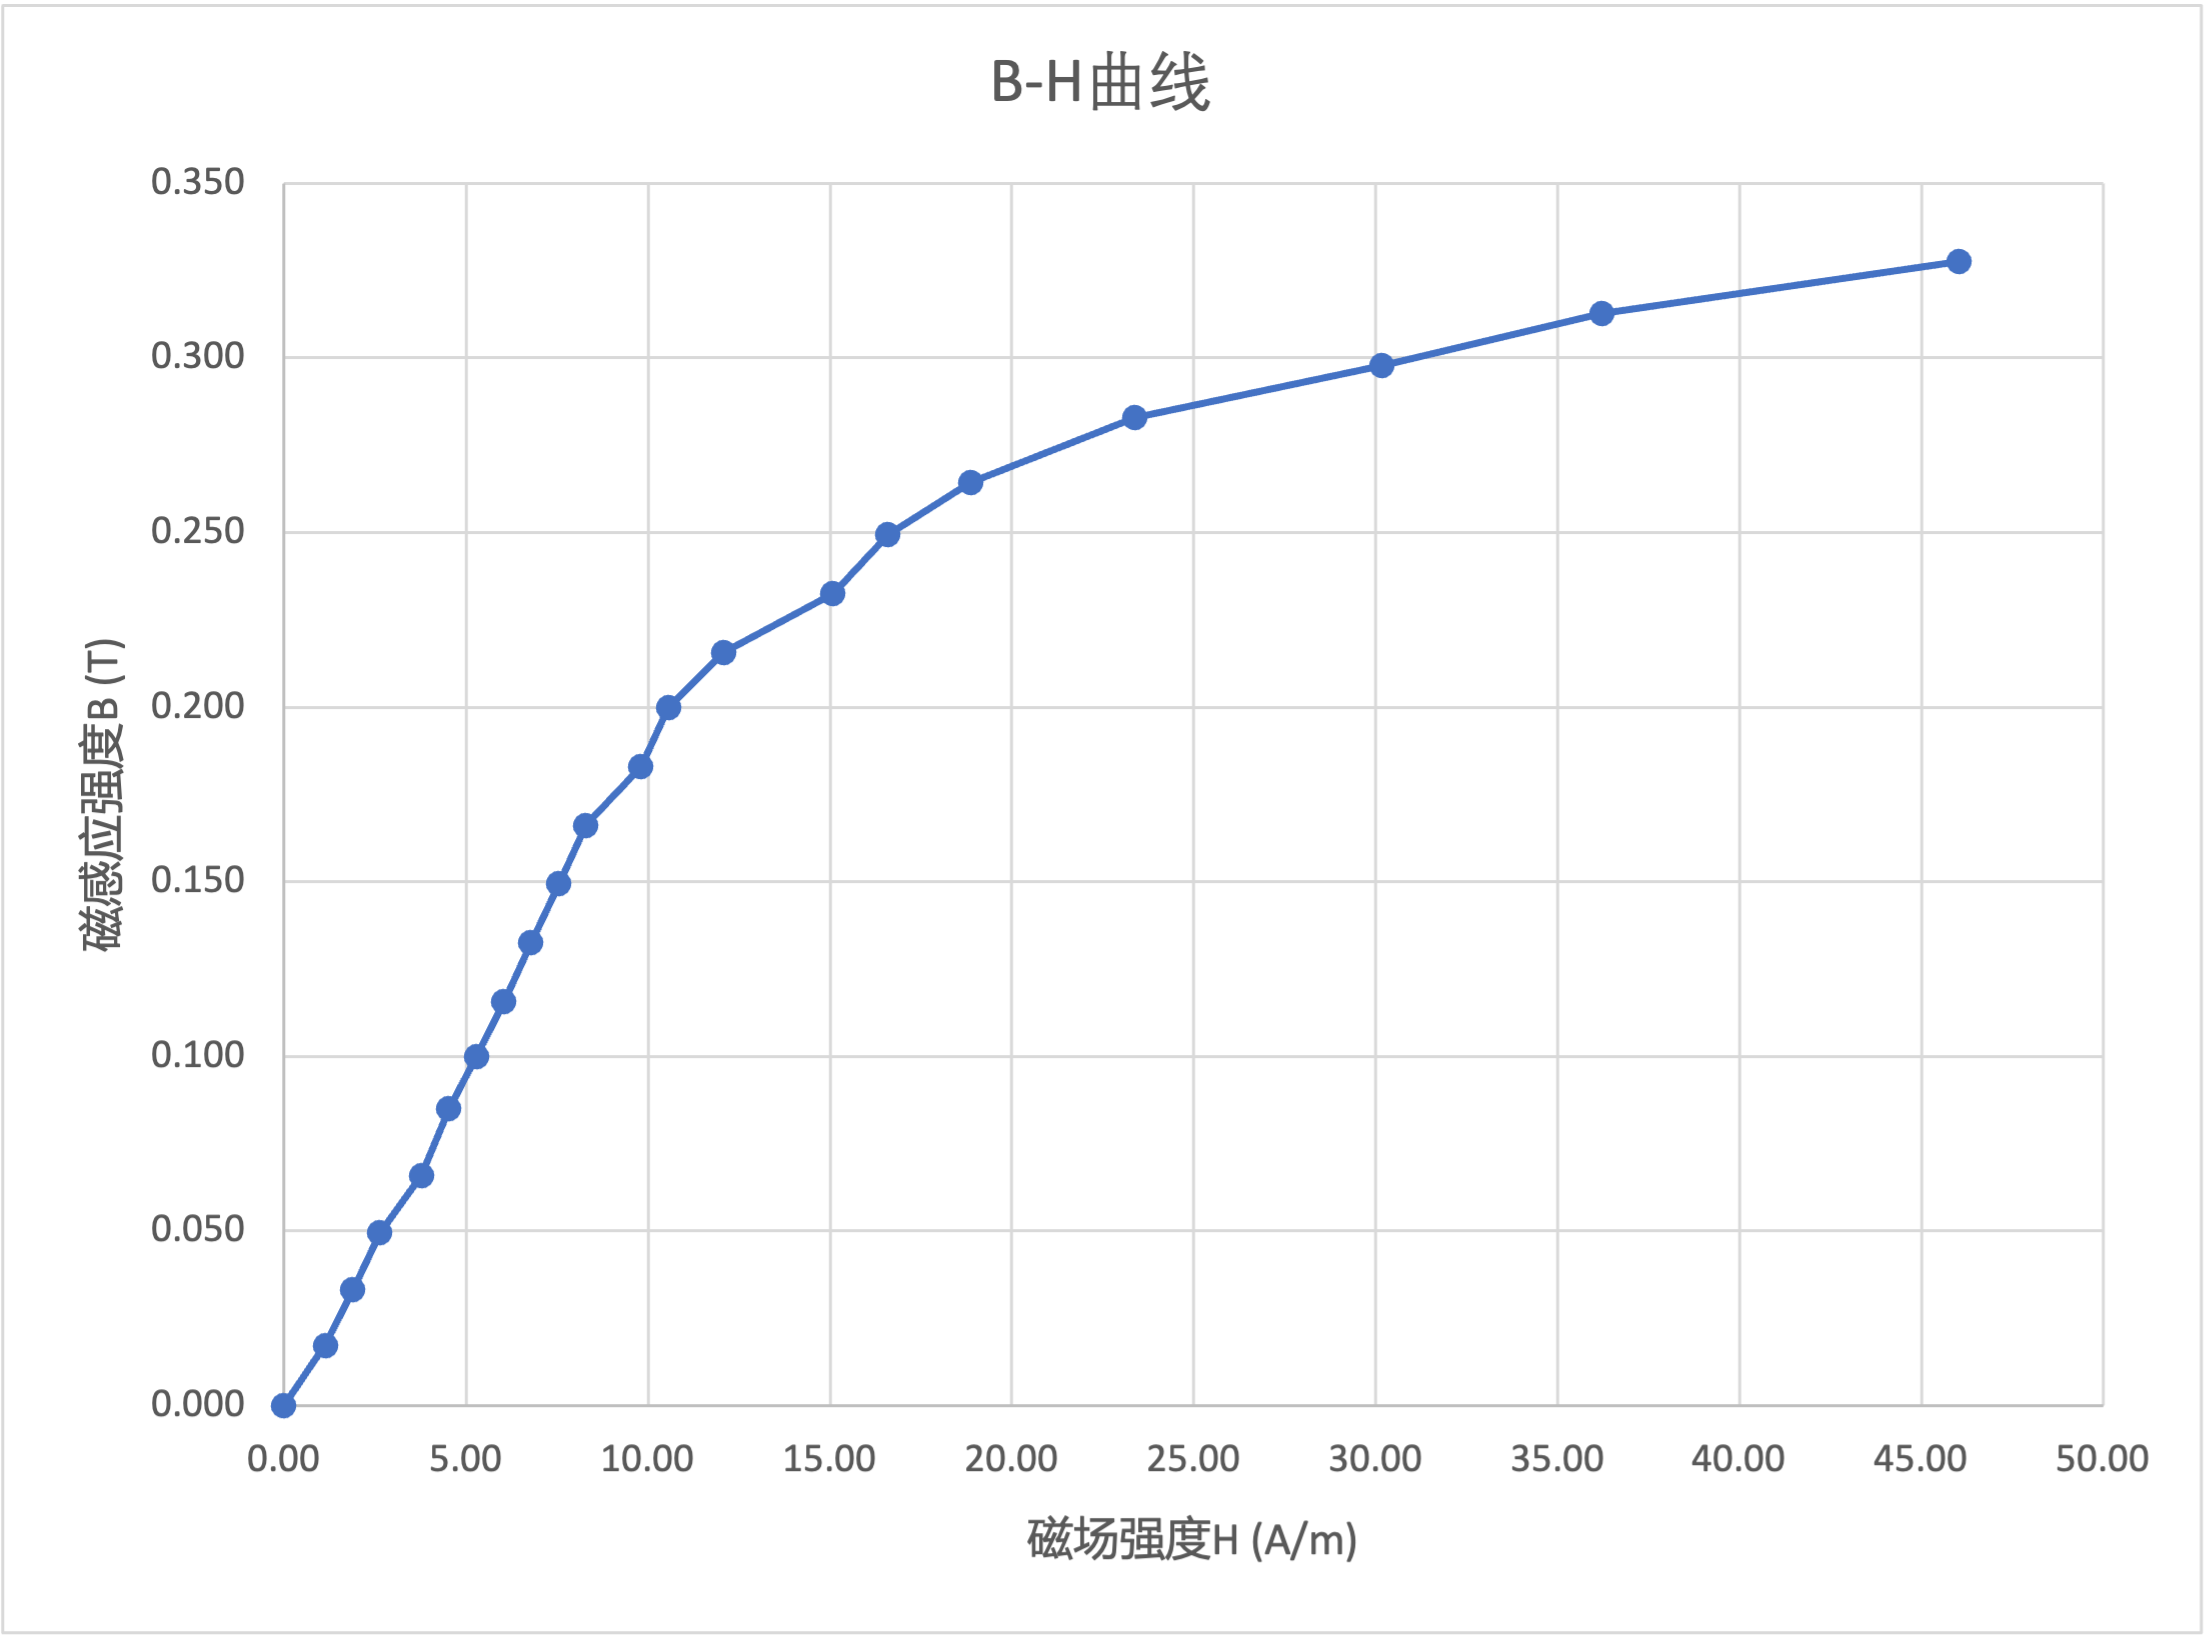
\includegraphics[width=1.0\textwidth]{plot11.png}
    \caption{样品的基本磁化曲线}
\end{figure*}

其中$H, B$的计算方法详见下文。

\subsection{$\mu-H$关系曲线}
已知常量:
\begin{itemize}
    \item $D_{inside} = 15 mm$
    \item $D_{outside} = 25.5 mm$
    \item $h = 10 mm$
    \item $C = 4.7 \mu F$
    \item $N_1 = N_2 = 120$
    \item $R_1 = 100 \Omega$
\end{itemize}
测得的横坐标记为$U_{R1}$,单位为$mV$;测得的纵坐标记为$U_C$,单位为$mV$;测得滑动变阻器$R_2 = 0.33154 k\Omega$。

$\mu, B, H$的计算方法如下:
\begin{align*}
    B &= \frac{R_2 \cdot C \cdot U_C}{N_2 S} \\
    H &= \frac{N_1 U_{R1}}{R_1 L} \\
    \mu &= \frac{B}{H}
\end{align*}

其中:
\begin{align*}
    L &= \frac{\pi (D_{inside} + D_{outside})}{2} \\
    &= \frac{3.14 \times (25.5 \times 10^{-3} + 15 \times 10^{-3})}{2} \\
    &= 0.0636 m \\
    S &= \frac{h (D_{outside} - D_{inside})}{2} \\
    &= \frac{10\times 10^{-3} \times (25.5 \times 10^{-3} - 15 \times 10^{-3})}{2} \\
    &= 5.25 \times 10^{-5} m^2
\end{align*}

计算结果如下:
\begin{figure*}[htbp]
    \centering
    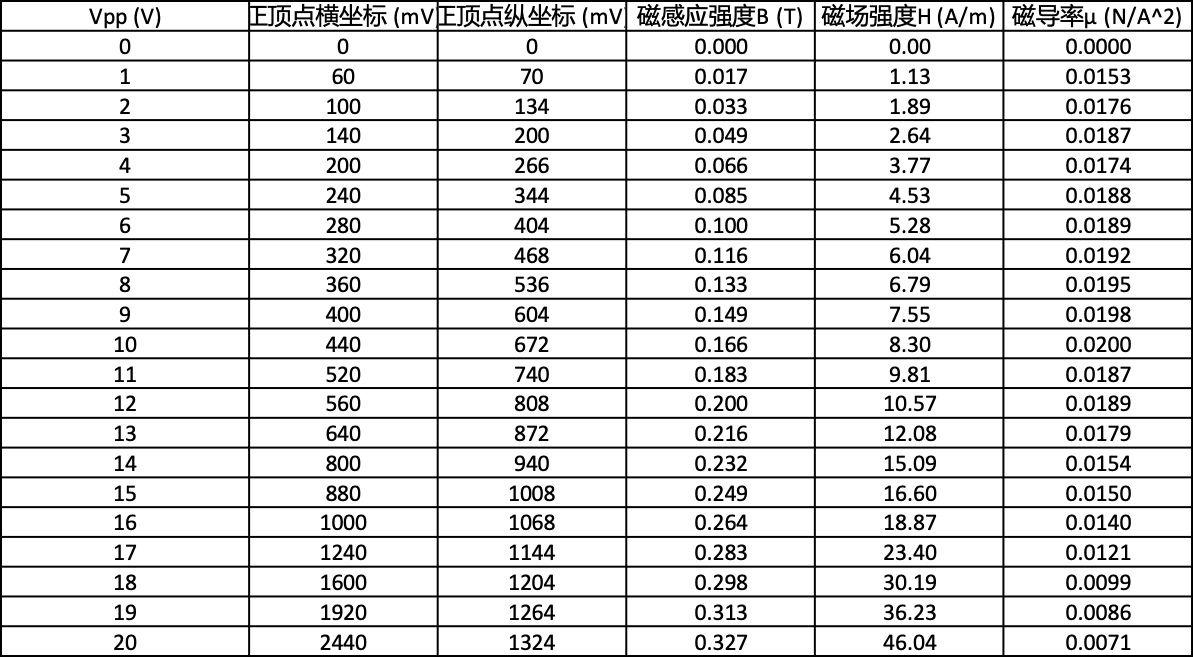
\includegraphics[width=1.0\textwidth]{data1.png}
    \caption{测量数据及磁导率、磁场强度计算结果}
\end{figure*}

绘制$\mu - H$曲线:
\begin{figure*}[htbp]
    \centering
    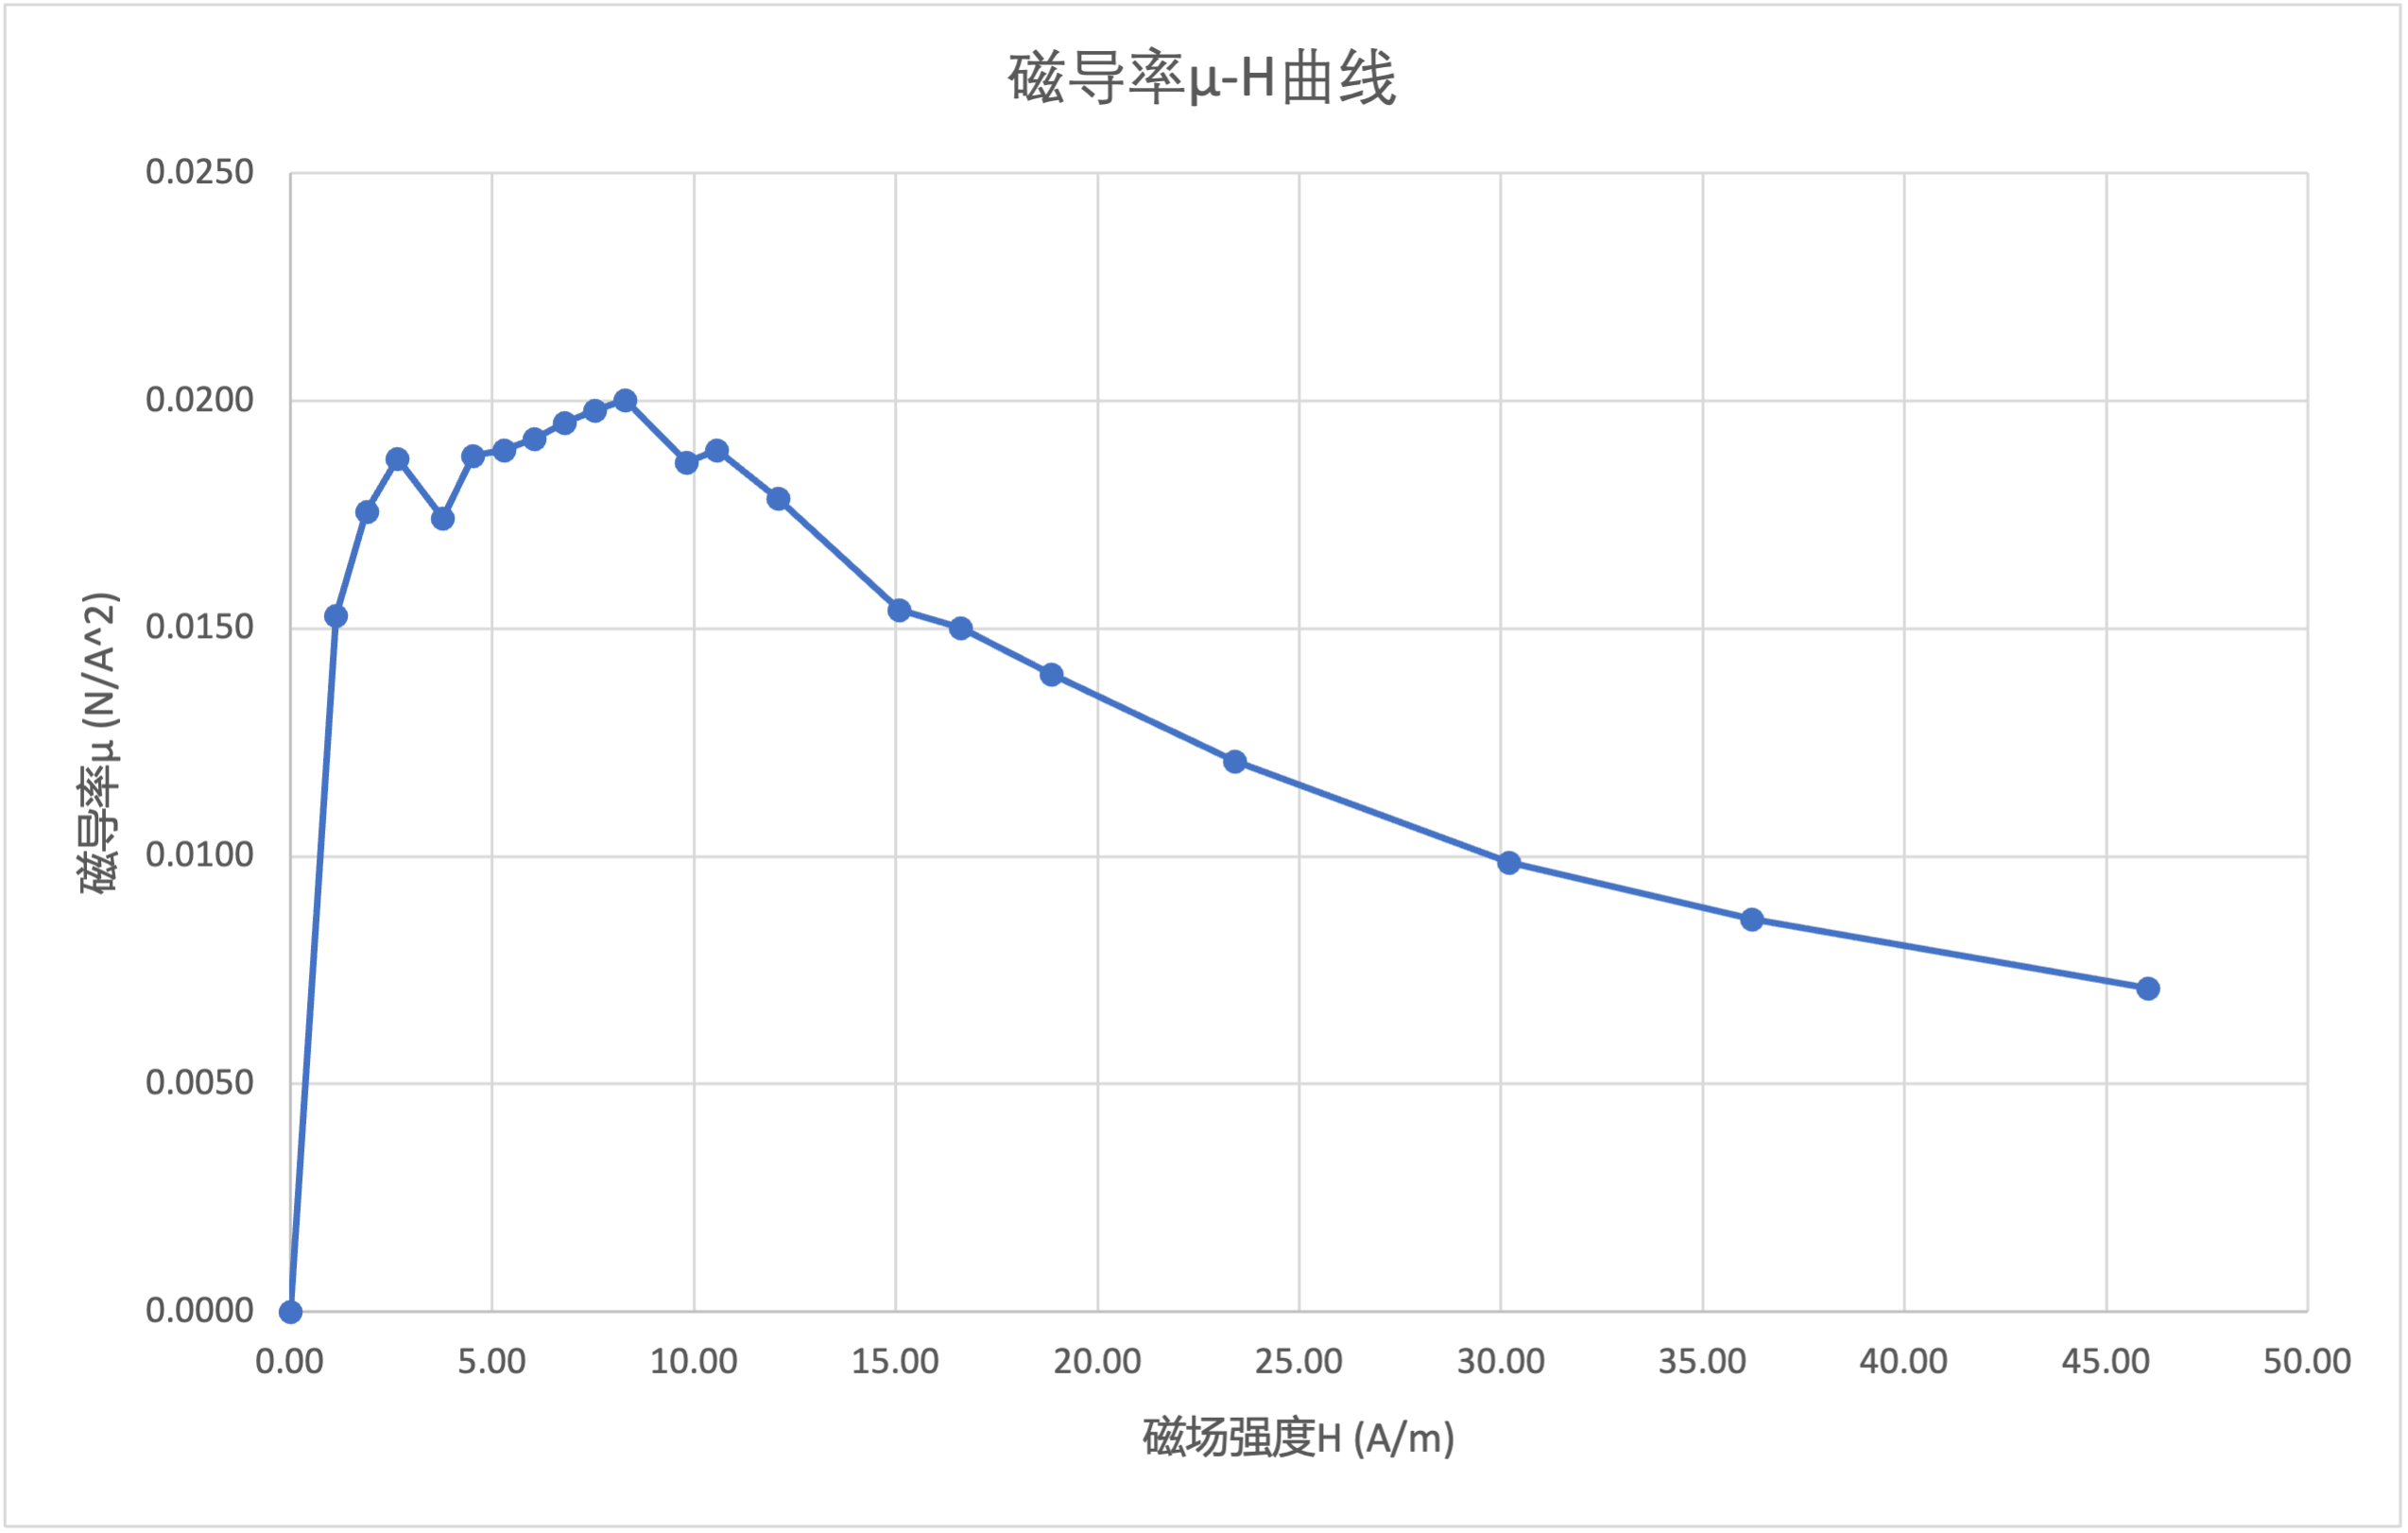
\includegraphics[width=1.0\textwidth]{plot2.png}
    \caption{磁导率$\mu$-磁场强度$H$关系曲线}
\end{figure*}

\newpage

\section{测绘磁滞回线}
利用同样的方法,根据测得的横纵坐标计算磁感应强度$B$和磁场强度$H$,计算结果如下:

\begin{figure*}[htbp]
    \centering
    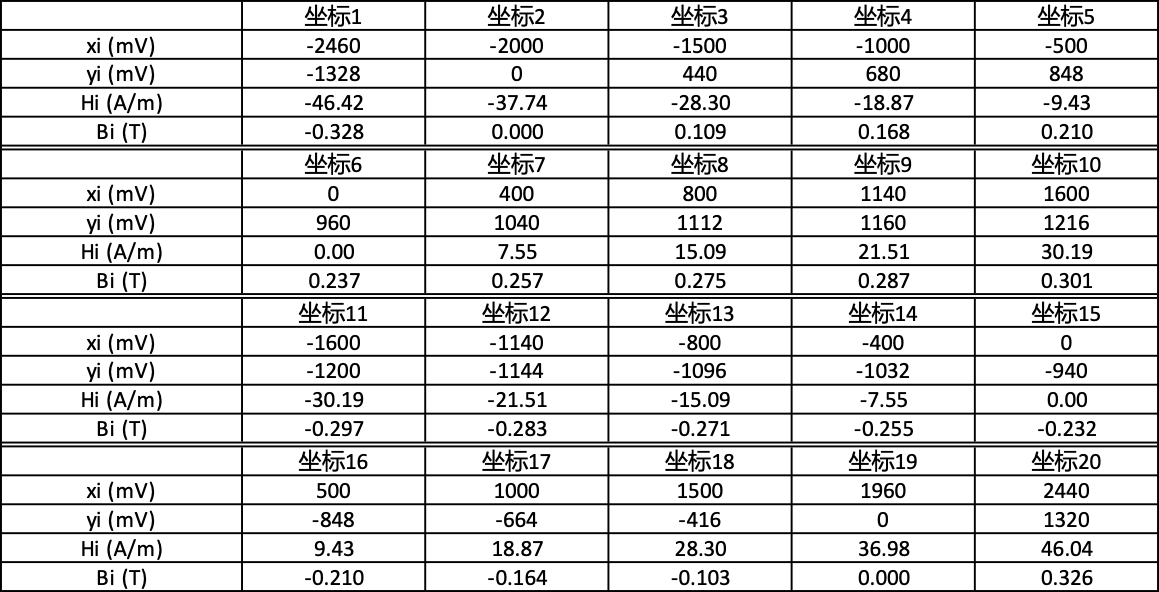
\includegraphics[width=1.0\textwidth]{data2.png}
    \caption{测量数据及磁感应强度、磁场强度计算结果}
\end{figure*}

共取了20个坐标点,其中坐标1, 2, 7, 16, 19, 20(已标红)为特殊点坐标,分别对应$(-Hs, -Bs), (-Hc, 0), (0, Br), (0, -Br), (Hc, 0), (Hs, Bs)$

绘制$B-H$曲线:
\begin{figure*}[htbp]
    \centering
    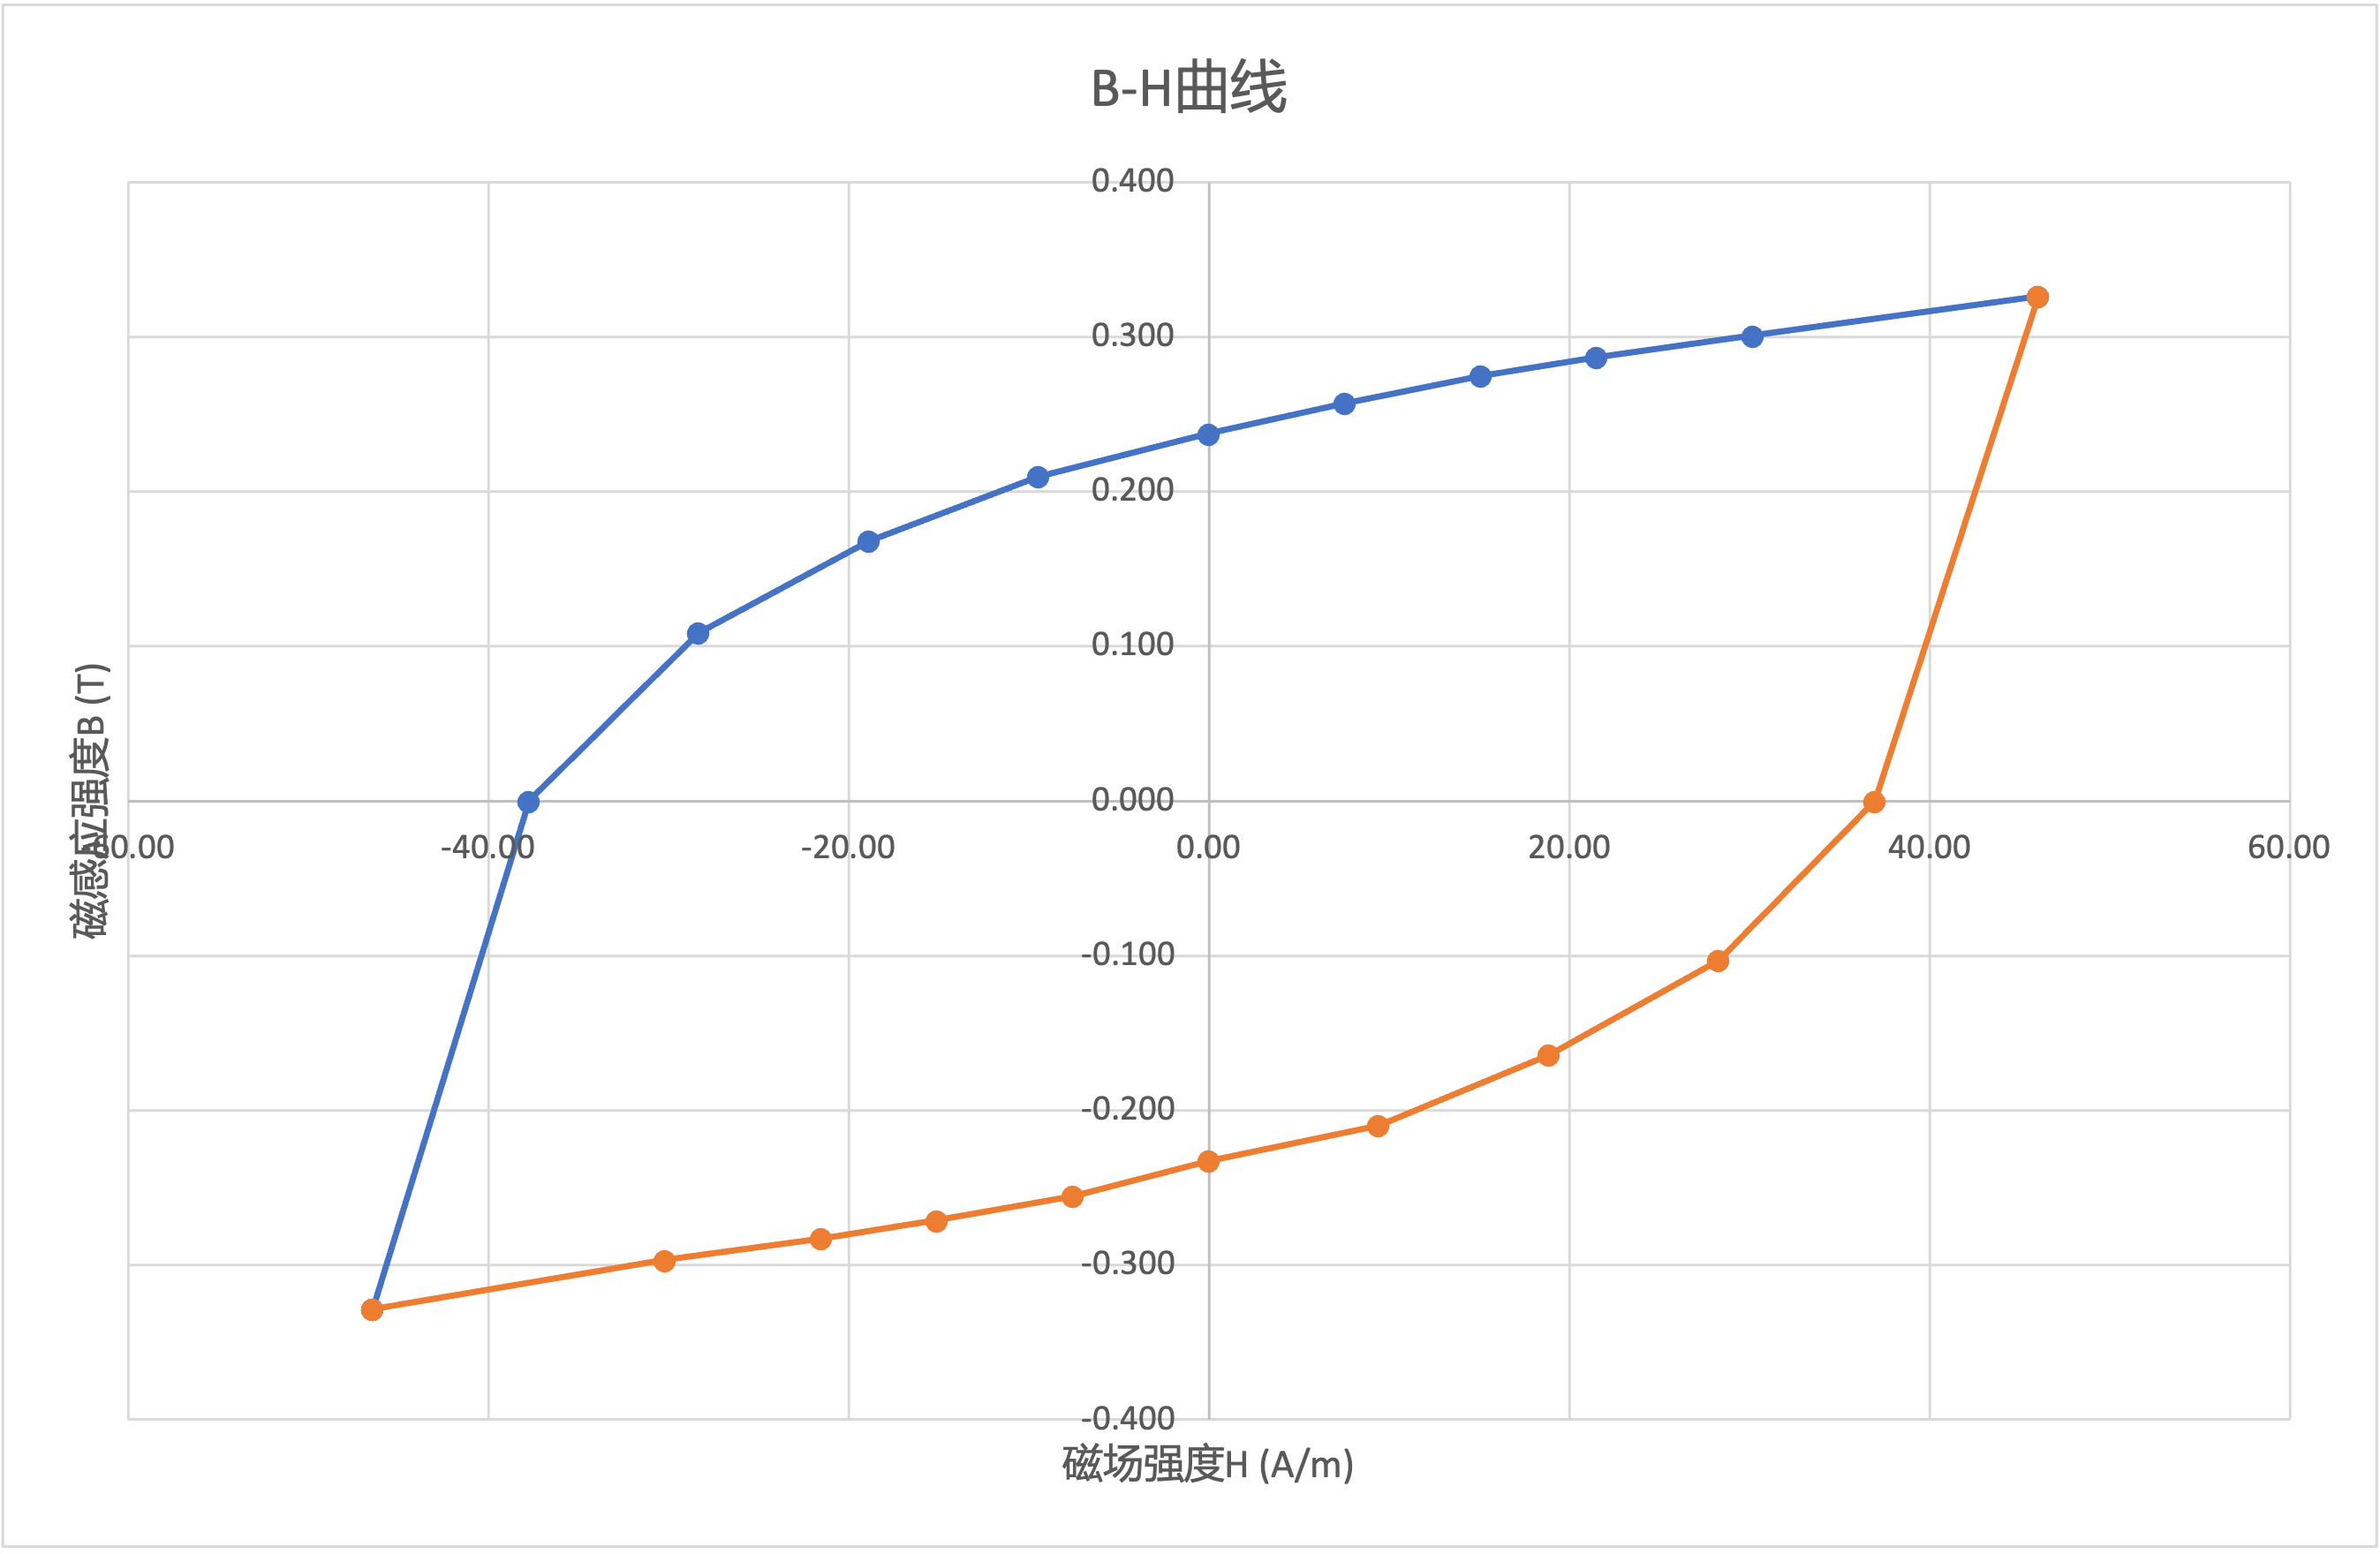
\includegraphics[width=1.0\textwidth]{plot3.png}
    \caption{样品的磁滞回线}
\end{figure*}

\newpage

\section{思考题}
\subsection{除了讲义中给出的方法,还有什么办法可以实现样品的完全退磁?}
\begin{itemize}
    \item 将磁性材料加热到其居里温度以上,然后在无外部磁场的环境下缓慢冷却。居里温度是铁磁材料从铁磁性转变为顺磁性的温度,加热至此温度会破坏材料内部的磁畴结构,使其失去磁性。缓慢冷却确保不会因冷却过程中的外部磁场重新磁化。
    \item 通过交变磁场影响磁畴的取向,逐步使其随机分布,达到退磁的目的。首先,应用一个足够大的交变磁场,使材料达到饱和磁化状态。然后,逐渐减小磁场的强度,并同时改变其方向,直到磁场的强度降低到零。
    \item 使用特制的退磁线圈,其通过线圈产生一个强大且方向不断变化的交变磁场。通过将磁性材料置于这样的磁场中,并逐渐减小磁场强度至零,可以有效地实现退磁。 
\end{itemize}

\subsection{可否用直流电的办法测量出磁滞回线?请简要设计一个测量方案。}
直流电不能直接产生交变磁场,但可以通过改变直流电的大小和方向来模拟磁场的变化。

从0开始,逐渐增加通过线圈的直流电流。每次增加一定量的电流,用霍尔效应传感器测量样品的磁感应强度 B。记录下每一步的电流值和相应的$B$值。

当电流增加到足以饱和样品的磁化时,逐渐减小电流直到零,再改变电流方向,重复增加电流的步骤,直到再次饱和样品的磁化。这一过程中,继续记录下电流值和相应的$B$值。

在达到饱和磁化后,再次减少电流直到零,然后逆向增加电流,重复以上步骤。

利用记录的电流值,可以计算出对应的磁场强度$H$和磁感应强度$B$值,绘制出磁滞回线图。

\section{分析与讨论}
\begin{itemize}
    \item 连接电路时,需要区分待测样品的接入端和接出端
    \item 通过将待测点移到原点的方式,读取李萨如图像中关键点的坐标,注意区分正负
    \item 测绘基本磁化曲线时,可以通过调整示波器的scale,调整到细长的形状,从而更清晰的观察到正顶点,但是这样会让测量精确度有所下降
    \item 测绘磁滞回线时,对于两条曲线都均匀的取点读取坐标,可以设定一系列横坐标点值然后找到对应纵坐标
\end{itemize}

\end{document}